\documentclass{article}
\usepackage[utf8]{inputenc}
\usepackage[english]{babel}
\usepackage[margin=1in]{geometry}
\usepackage{titlesec}
\usepackage{fancyhdr}
\usepackage[hidelinks]{hyperref}
\usepackage{tikz}
\usepackage{fancyhdr}
\usepackage{float}
\usetikzlibrary{trees}
\author{R\'emy Detobel \& Nathan Liccardo}
\title{Report : XML Schema Definition}

\renewcommand\thesection{\arabic{section}}

\begin{document}

\maketitle

\section{Introduction}
The aims of this document will be to describe and explain all the choices that we made for our project. To call back, the main goal of this assignment was to create an XSD file which contains a specific XML Schema Definition. The first part of this report will be dedicated to the structure of the schema. We will show, by means of trees, how the requested structure has been implemented. Those trees will be used to infer each specific types and links between them. The second part of this document will be focused on the hypotheses that we made during the implementation. All those choices were made arbitrarily and can be changed

\section{Structure of the schema}
One of the solution to define an XML Schema is to use an XSD file. This file will contain all the relations between elements but also the restrictions applied to each types (simple or complex). For this project, we were assigned to write an XSD file which define a book shop. This shop is separated into two parts : scientific products and leisure products. The following tree represent this first relation : 
\begin{center}
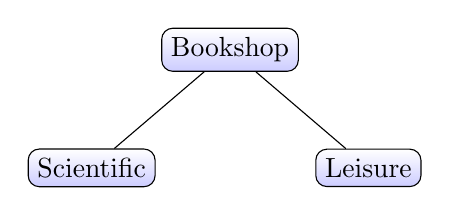
\begin{tikzpicture}[sibling distance=10em,
  every node/.style = {shape=rectangle, rounded corners,
    draw, align=center,
    top color=white, bottom color=blue!20}]]
  \node {Bookshop}
    child { node {Scientific} }
    child { node {Leisure} };
\end{tikzpicture}
\end{center}

\subsection{Scientific products}
Scientific products are separated into two sub-categories. The first one define scientific books and the second one scientific journals. Those links can be represented as follow :  
\begin{center}
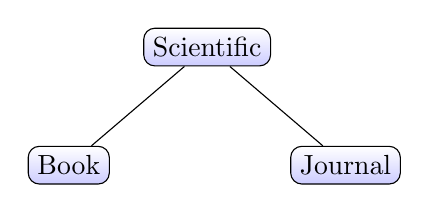
\begin{tikzpicture}[sibling distance=10em,
  every node/.style = {shape=rectangle, rounded corners,
    draw, align=center,
    top color=white, bottom color=blue!20}]]
  \node {Scientific}
    child { node {Book} }
    child { node {Journal} };
\end{tikzpicture}
\end{center}
Based on this, we can define multiple relations. Those relations will be used to represent complex types in the XSD file. As shown in the previous tree, we can define three complex types named scientificType, bookType and journalType :
\begin{itemize}
\item bookshopType $\rightarrow$ (scientific, scientificType)
\item scientificType $\rightarrow$ (book, booktype1), (journal, journalType)
\end{itemize}
For the moment, we are not going to define the bookshopType. In fact, we do not have enough informations to define it correctly now. We are so assuming that it is an abstract type. Regarding the two final complex types, called bookType and journalType, a complete explanation of these will be given in the second part dedicated to hypotheses and choices.

\subsection{Leisure products}
The second section of a book shop is dedicated to leisure products. As for scientific one, products are separated into two sub-categories. The first one is used to define leisure books and the second one leisure periodicals. Once again , those links can be illustrated by means of a tree : 
\begin{center}
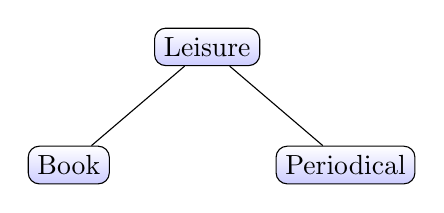
\begin{tikzpicture}[sibling distance=10em,
  every node/.style = {shape=rectangle, rounded corners,
    draw, align=center,
    top color=white, bottom color=blue!20}]]
  \node {Leisure}
    child { node {Book} }
    child { node {Periodical} };
\end{tikzpicture}
\end{center}
Following this tree, we can obtain two relations. These last are used to define an abstract bookshop (bookshopType) and a final leisure (leisureType). Finally, we obtain the next definitions :
\begin{itemize}
\item bookshopType $\rightarrow$ (leisure, leisureType)
\item leisureType $\rightarrow$ (book, booktype2), (periodical, periodicalType)
\end{itemize}
As said in the previous sub-section, bookshopType is actually not completely defined. For this reason, there exist some incompatibilities between the scientific and leisure part. Notice that leisure books and scientific books are not using same types. In fact we will see in the next section that they have two different definitions.

\subsection{Complete schema}
The two previous parts were focused on the scientific and leisure definitions. We have now to merge those definitions to obtain the final tree. In fact, a bookshop is a combination of scientific and leisure products. Notice that for each element (book, journal, ...) we can also have multiple instances of it. Finally, we obtain the following tree :
\begin{center}
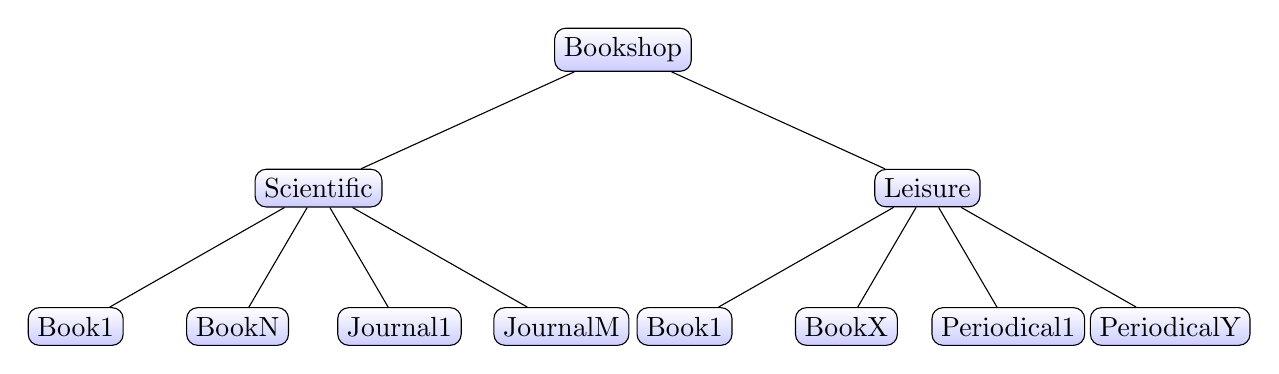
\begin{tikzpicture}[level distance=5em,
	level 1/.style={sibling distance=22em},
  level 2/.style={sibling distance=5.85em},
  every node/.style = {shape=rectangle, rounded corners,
    draw, align=center,
    top color=white, bottom color=blue!20}]]
  \node{Bookshop}  
    child { node {Scientific}
    	child { node {Book1} }
	child { node {BookN} }
    	child { node {Journal1} }
	child { node {JournalM} } }  
    child { node {Leisure}
    	child { node {Book1} }
    	child { node {BookX} }
    	child { node {Periodical1} }
    	child { node {PeriodicalY} } };
\end{tikzpicture}
\end{center}
Previously, we defined the bookshopType as an abstract one. In fact, this type was a sequence of scientificType and leisureType and could not be defined in one time. As we changed the definition of a bookshopType but also of a scientificType and a leisureType, we obtain three new relations :
\begin{itemize}
\item bookshopType $\rightarrow$ (scientific, scientificType),(leisure, leisureType)
\item scientificType $\rightarrow$ (book, booktype1)*, (journal, journalType)*
\item leisureType $\rightarrow$ (book, booktype2)*, (periodical, periodicalType)*
\end{itemize}
For the moment, we only defined links between elements. All those are created by defining complex types with some elements inside. Each of these elements are themselves referring to other complex type excepted for final types (Book, Journal, ...). The second part of this report will be focused on explaining and illustrating all the choices that we made during the implementation. For this reason, we will also detail the structure of each final types.

\end{document}